\section{Observations}
\markright{Observations}

The diode current was calculated from the voltage drop across the series resistor:
\[
    I_D = \frac{V_S - V_D}{10\,\text{k}\Omega}
\]
For forward bias the result is expressed in mA, and for reverse bias it is expressed in
$\mu$A.

\subsection*{Forward Bias Observation}

\begin{table}[H]
    \centering
    \caption{Observed forward-bias readings for the silicon p-n junction diode}
    \label{tab:lab2_forward_observation}
    \renewcommand{\arraystretch}{1.45}
    \setlength{\tabcolsep}{9pt}
    \begin{tabular}{|c|c|c|c|}
        \hline
        \textbf{S. No.} & \textbf{Applied Voltage (V)} & \textbf{$V_F$ (V)} & \textbf{$I_F$ (mA)} \\
        \hline
        1 & 0.1 & 0.10 & 0.000 \\
        \hline
        2 & 0.3 & 0.29 & 0.001 \\
        \hline
        3 & 0.5 & 0.39 & 0.011 \\
        \hline
        4 & 0.7 & 0.43 & 0.027 \\
        \hline
        5 & 0.9 & 0.45 & 0.045 \\
        \hline
        6 & 1.1 & 0.46 & 0.064 \\
        \hline
        7 & 1.3 & 0.47 & 0.083 \\
        \hline
        8 & 1.5 & 0.48 & 0.102 \\
        \hline
    \end{tabular}
\end{table}

\subsection*{Reverse Bias Observation}

\begin{table}[H]
    \centering
    \caption{Observed reverse-bias readings for the silicon p-n junction diode}
    \label{tab:lab2_reverse_observation}
    \renewcommand{\arraystretch}{1.45}
    \setlength{\tabcolsep}{9pt}
    \begin{tabular}{|c|c|c|c|}
        \hline
        \textbf{S. No.} & \textbf{Applied Voltage (V)} & \textbf{$V_R$ (V)} & \textbf{$I_R$ ($\mu$A)} \\
        \hline
        1 & 2 & 1.98 & 2.00 \\
        \hline
        2 & 4 & 3.96 & 4.00 \\
        \hline
        3 & 5 & 4.95 & 5.00 \\
        \hline
        4 & 8 & 7.92 & 8.00 \\
        \hline
        5 & 9 & 8.93 & 7.00 \\
        \hline
        6 & 10 & 9.90 & 10.00 \\
        \hline
        7 & 11 & 10.89 & 11.00 \\
        \hline
        8 & 11.5 & 11.39 & 11.00 \\
        \hline
    \end{tabular}
\end{table}

\begin{figure}[H]
    \centering
    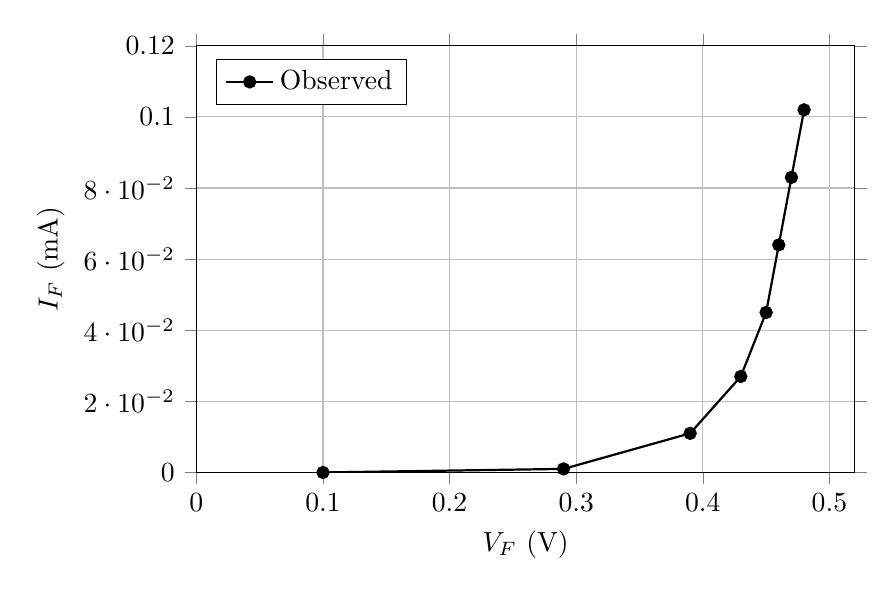
\begin{tikzpicture}
        \begin{axis}[
            width=0.82\textwidth,
            height=7cm,
            grid=both,
            xlabel={$V_F$ (V)},
            ylabel={$I_F$ (mA)},
            xmin=0, xmax=0.52,
            ymin=0, ymax=0.12,
            tick align=outside,
            legend pos=north west
        ]
            \addplot[
                mark=*,
                thick
            ] coordinates {
                (0.10,0.000)
                (0.29,0.001)
                (0.39,0.011)
                (0.43,0.027)
                (0.45,0.045)
                (0.46,0.064)
                (0.47,0.083)
                (0.48,0.102)
            };
            \addlegendentry{Observed}
        \end{axis}
    \end{tikzpicture}
    \caption{Observed forward V--I characteristic of the silicon p-n junction diode.}
    \label{fig:lab2_observed_forward_vi}
\end{figure}

\begin{figure}[H]
    \centering
    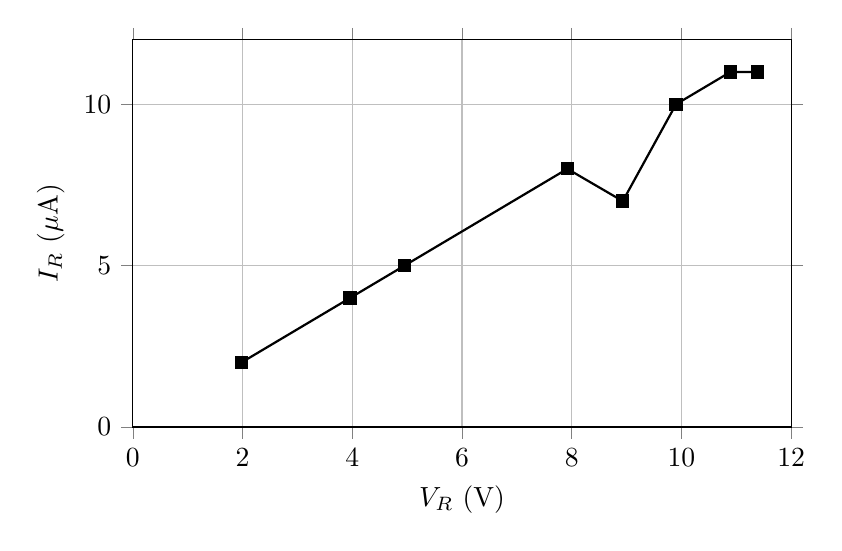
\begin{tikzpicture}
        \begin{axis}[
            width=0.82\textwidth,
            height=6.5cm,
            grid=both,
            xlabel={$V_R$ (V)},
            ylabel={$I_R$ ($\mu$A)},
            xmin=0, xmax=12,
            ymin=0, ymax=12,
            tick align=outside
        ]
            \addplot[
                mark=square*,
                thick
            ] coordinates {
                (1.98,2.00)
                (3.96,4.00)
                (4.95,5.00)
                (7.92,8.00)
                (8.93,7.00)
                (9.90,10.00)
                (10.89,11.00)
                (11.39,11.00)
            };
        \end{axis}
    \end{tikzpicture}
    \caption{Observed reverse V--I characteristic of the silicon p-n junction diode.}
    \label{fig:lab2_observed_reverse_vi}
\end{figure}
